\chapter{UEFI, BIOS and platform}
\begin{note}[Abbreviations]:\\
	\begin{table}[h]
	\makegapedcells
	\centering
	\resizebox{\textwidth}{!}{%resizing the whole table
\begin{tabular}{|c|P{13cm}|}\hline
\textbf{Abbreviation} & \textbf{Meaning} \\  \hline

\href{https://en.wikipedia.org/wiki/Advanced_Configuration_and_Power_Interface}{\textbf{ACPI}} & Advanced Configuration and Power Interface \\   \hline
\href{https://en.wikipedia.org/wiki/Advanced_Programmable_Interrupt_Controller}{\textbf{APIC}} & Advanced Programmable Interrupt Controller \\   \hline
\href{https://en.wikipedia.org/wiki/Direct_memory_access}{\textbf{DMA}} & Direct Memory Access \\   \hline
\href{https://en.wikipedia.org/wiki/Direct_Media_Interface}{\textbf{DMI}} & Direct Media Interface \\   \hline
\href{https://en.wikipedia.org/wiki/EFI_system_partition}{\textbf{ESP}} & EFI System Partition \\   \hline
\href{https://www.dataman.com/media/datasheet/Intel/82802Ax.pdf}{\textbf{FWH}} & Firmware Hub \\   \hline
\href{https://en.wikipedia.org/wiki/GUID_Partition_Table}{\textbf{GPT}} & GUID Partition Table \\   \hline
\href{https://en.wikipedia.org/wiki/I/O_Controller_Hub}{\textbf{ICH}} & I/O Controller Hub (Southbridge)\\   \hline
\href{https://en.wikipedia.org/wiki/Industry_Standard_Architecture}{\textbf{ISA}} & Industry Standard Architecture\\   \hline
\href{https://en.wikipedia.org/wiki/Low_Pin_Count}{\textbf{LPC}} & Low Pin Count \\   \hline
\href{https://en.wikipedia.org/wiki/Northbridge_(computing)}{\textbf{MCH}} & Memory Controller Hub (Northbridge)\\   \hline
\href{https://en.wikipedia.org/wiki/Platform_Controller_Hub}{\textbf{PCH}} & Platform Controller Hub\\   \hline
\href{https://en.wikipedia.org/wiki/Conventional_PCI}{\textbf{PCI}} & Peripheral Component Interconnect\\   \hline
\textbf{PEIM} & Pre EFI Initialization Module\\   \hline
\href{https://en.wikipedia.org/wiki/System_Management_Bus}{\textbf{SMBus}} & System Management Bus \\   \hline
\href{https://en.wikipedia.org/wiki/System_Management_Mode}{\textbf{SMI}} & System Management Interrupt \\   \hline
\href{https://en.wikipedia.org/wiki/System_Management_Mode}{\textbf{SMM}} & System Management Mode \\   \hline
\href{https://en.wikipedia.org/wiki/Serial_Peripheral_Interface}{\textbf{SPI}} & Serial Peripheral Interface \\   \hline
\href{https://en.wikipedia.org/wiki/Trusted_Platform_Module}{\textbf{TPM}} & Trusted Platform Module \\   \hline
\href{https://www.uefi.org/}{\textbf{UEFI}} & Unified Extensible Firmware Interface \\   \hline
\end{tabular}
}
\caption{UEFI and platform abbreviations}
\end{table}

\end{note}
\section[GPT]{GPT\protect\footnote{GUID Partition Table}}
\begin{tabularx}{\textwidth}[t]{p{0.4\textwidth}rN}
 & \multirow{2}{*}{\includegraphics[scale=0.8]{Images/UEFI/GUIDPartitionTableScheme}} \\ 
 \begin{itemize}
 	\item GUID Partition Table (GPT) is a standard for the layout of the partition table on a physical storage device and it forms a part of the Unified Extensible Firmware Interface (UEFI) standard.
 	\item The GUID for an EFI system partition is C12A7328-F81F-11D2-BA4B-00A0C93EC93B
 	\item The Partition Entry Array describes partitions, using a minimum size of 128 bytes for each entry block.
 	\item Secondary GPT is nothing but a backup for Primary GPT
 \end{itemize} \\ [11cm]
\end{tabularx}

\begin{table}[h]
\begin{center}
	\begin{tabular}{|c|l|l|}\hline
		\multicolumn{1}{c}{ \bfseries Offset} & \multicolumn{1}{c}{\bfseries Length} & \multicolumn{1}{c}{\bfseries Contents} \\ \hline 
		0 (0x00) & 16 bytes & Partition type GUID \\ \hline
		16 (0x10)&	16 bytes&	Unique partition GUID\\ \hline
		32 (0x20)&	8 bytes&	First LBA (little endian)\\ \hline
		40 (0x28)&	8 bytes&	Last LBA (inclusive, usually odd)\\ \hline
		48 (0x30)&	8 bytes&	Attribute flags (e.g. bit 60 denotes read-only)\\ \hline
		56 (0x38)&	72 bytes&	Partition name (36 UTF-16LE code units)\\ \hline
	\end{tabular}
\end{center}
	\caption{GPT Entries}
\end{table}


\section{PCI and PCI Express}
\begin{note}[General notes]:
\begin{itemize}
	\item PCI \footnote{Peripheral Component Interconnect} is a local computer bus for attaching hardware devices in a computer.
	\item Supersedes: ISA, EISA, MCA, VLB, Superseded by: PCI Express (2004)
	\item Since about 2005, the ISA slot is no longer installed in desktop PCs.
	\item The PCI Express bus extends the Configuration Space from 256 bytes to 4096 bytes. This extended configuration space *cannot* be accessed using the legacy PCI method (through ports 0xCF8 and 0xCFC)
\end{itemize}
\end{note}
\begin{note}[Configuration Space]:
	
The PCI specification provides for totally software driven initialization and configuration of each device (or target) on the PCI Bus via a separate Configuration Address Space. All PCI devices, except host bus bridges, are required to provide 256 bytes of configuration registers for this purpose.

PCI devices are inherently little-endian, meaning all multiple byte fields have the least significant values at the lower addresses. This requires a big-endian processor, such as a Power PC, to perform the proper byte-swapping of data read from or written to the PCI device, including any accesses to the Configuration Address Space.\\
\end{note}
\begin{note}[Configuration Space Access Mechanisms]:\\
\textbf{Configuration Space Access Mechanism \#1}:
\begin{itemize}
	\item Two 32-bit I/O locations are used, the first location (0xCF8) is named \verb|CONFIG_ADDRESS|, and the second (0xCFC) is called \verb|CONFIG_DATA|. 
	
\begin{table}[h]
\begin{center}
	\begin{tabular}{|c|c|c|c|c|c|c|}\hline
		31 & 30 - 24 & 23 - 16 & 15 - 11 & 10 - 8 & 7 - 2 &1 - 0 \\ \hline 
		Enable Bit & Reserved & Bus Number & Device Number & Function Number & Register Number & 00\\ \hline 
	\end{tabular}
\end{center}
	\caption{PCI Config Address Register}
\end{table}


	\item Python script for translation:
\begin{lstlisting}[language=Python]
BITMASK = lambda reg, higher,lower:
	(reg >> lower) & (2 ** (higher-lower+1) - 1)

def IO_PORT_CONFIG_ADDRESS_COMPONENTS(address):
	register = BITMASK(address,7,2)
	function = BITMASK(address,10,8)
	device   = BITMASK(address,15,11)
	bus      = BITMASK(address,23,16)
	reserved = BITMASK(address,30,24)
	enabled  = BITMASK(address,31,31)
	if address & 3 != 0 or reserved != 0:
		print ("Invalid address")
		return
	print ("Register: 0x%X Function: 0x%X Device: 0x%X" +
	       "Bus: 0x%X Enabled: 0x%X" % 
	       (register, function, device, bus, enabled))
\end{lstlisting}
\end{itemize}
\textbf{Configuration Space Access Mechanism \#2}:

\href{https://wiki.osdev.org/PCI#Configuration_Space_Access_Mechanism_.232}{This} configuration space access mechanism was deprecated in PCI version 2.0. This means it's only likely to exist on hardware from around 1992.\\
\textbf{Configuration Space Access Mechanism \#3 - Memory Mapped PCI Configuration Space Access}:
\begin{itemize}
	\item PCI Express introduced a new way to access PCI configuration space, where it's simply memory mapped and no IO ports are used.
	\item Systems that do provide the memory mapped access mechanism are also required to support PCI access mechanism \#1 for backward compatibility.
	\item The enhanced configuration mechanism makes use of memory mapped address space range/s to access PCI configuration space. Put simply, the memory address determines the segment group, bus, device, function and register being accessed. On x86 and x64 platforms, the address of each memory area is determined by the ACPI 'MCFG' table.
	\item To find 'MCFG', Search the ACPI Root System Descriptor Table(RSDT) or Extended Root System Descriptor Table(XSDT)
	\item $Physical Address = MMIO Starting Physical Address + ( (Bus - MMIO Starting Bus) << 20 | Device << 15 | Function << 12 )$
\end{itemize}

\begin{table}[h]
	\centering
	\begin{tabular}{|c|c|c|c|l|N|}\hline
		\multicolumn{1}{c}{ \bfseries Offset} & \multicolumn{1}{c}{\bfseries Length} & \multicolumn{3}{c}{\bfseries Description} \\ \hline 
		0 & 4 & \multicolumn{3}{l}{Table Signature ("MCFG")} &\\ \hline
		4 & 4 & \multicolumn{3}{l}{Length of table (in bytes)} &\\ \hline
		8 & 1 & \multicolumn{3}{l}{Revision (1)} &\\ \hline
		9 & 1 & \multicolumn{3}{l}{Table SignatureChecksum (sum of all bytes in table \& 0xFF = 0)} &\\ \hline
		10 & 6 & \multicolumn{3}{l}{OEM ID (same meaning as other ACPI tables)} &\\ \hline
		16 & 6 & \multicolumn{3}{l}{OEM table ID (manufacturer model ID)} &\\ \hline
		24 & 4 & \multicolumn{3}{l}{OEM Revision (same meaning as other ACPI tables)} &\\ \hline
		28 & 4 & \multicolumn{3}{l}{Creator ID (same meaning as other ACPI tables)} &\\ \hline
		32 & 4 & \multicolumn{3}{l}{Creator Revision (same meaning as other ACPI tables)} &\\ \hline
		36 & 8 & \multicolumn{3}{l}{Reserved} &\\ \hline
		\multirow{7}{*}{44} & \multirow{7}{*}{16 * n} & \multicolumn{3}{l}{Configuration space base address allocation structures.} &\\ \cline{3-5}
		&& \bfseries Offset & \bfseries Length & \multicolumn{1}{c}{\bfseries Description} &\\ \cline{3-5}
		&& 0 & 8 & Base address of enhanced configuration mechanism &\\ \cline{3-5}
		&& 8 & 2 & PCI Segment Group Number &\\ \cline{3-5}
		&& 10 & 1 & Start PCI bus number decoded by this host bridge &\\ \cline{3-5}
		&& 11 & 1 & End PCI bus number decoded by this host bridge &\\ \cline{3-5}
		&& 12 & 4 & Reserved &\\ \hline
	\end{tabular}
	\caption{MCFG Table}
\end{table}


\begin{lstlisting}[language=Python]
def PCI_LIB_ADDRESS_COMPONENTS(address):
	register = address & 0xfff
	function = (address >> 12) & 0x7
	device = (address >> 15) & 0x1f
	bus = (address >> 20) & 0xff
	extend = (address >> 28)
	
	print ("Register: 0x%X Function: 0x%X " +
	       "Device: 0x%X Bus: 0x%X Extend: 0x%X" %
	       (register, function, device, bus, extend))
\end{lstlisting}
\end{note}


\section{BIOS Flash Locations}
\begin{note}[Where bios is stored]:\\
BIOS can reside in one of 3 locations:
\begin{itemize}
	\item Firmware Hub (FWH) (Old technology)
	\item SPI Flash (most likely this is the case)
	\item PCI (intended for debugging or recovering from a corrupted BIOS, not supported anymore on newer hardware)
\end{itemize}

\end{note}
\begin{note}[Find BIOS boot destination]:
	
To programmatically find where your BIOS is configured to boot from, you can view bits 11:10 in the General Control and Status Register (GCS). It is located at memory mapped offsets 3410-3413h in the Chipset Configuration Registers and Chipset Configuration Registers are mapped starting at the address held by RCBA\footnote{Root Complex Base Address Register}
\end{note}

\begin{note}[SPI Flash]:
	
\end{note}

\section{UEFI Firmware Volume}
\begin{note}[File types]:
\begin{lstlisting}[language=C]
typedef UINT8 EFI_FV_FILETYPE;

#define EFI_FV_FILETYPE_RAW                   0x01
#define EFI_FV_FILETYPE_FREEFORM              0x02
#define EFI_FV_FILETYPE_SECURITY_CORE         0x03
#define EFI_FV_FILETYPE_PEI_CORE              0x04
#define EFI_FV_FILETYPE_DXE_CORE              0x05
#define EFI_FV_FILETYPE_PEIM                  0x06
#define EFI_FV_FILETYPE_DRIVER                0x07
#define EFI_FV_FILETYPE_COMBINED_PEIM_DRIVER  0x08
#define EFI_FV_FILETYPE_APPLICATION           0x09
#define EFI_FV_FILETYPE_FIRMWARE_VOLUME_IMAGE 0x0b
#define EFI_FV_FILETYPE_FFS_PAD               0xf0
\end{lstlisting}
\end{note}
\section{Reset Vector}
\begin{note}[Initial Bootstrap]:
\begin{itemize}
	\item EIP (or IP since it’s 16-bit mode) is initialized with (0000)FFF0	– CS:IP = F:FFF0h
	\item CR0 is 60000010h (likely since Pentium)
	\item Paging (bit 31) is disabled, Protection Enable (bit 0) is 0
	\item SPI flash is bootstrapped in top 16 MB memory (0xFF000000 to 0xFFFFFFFF)
	\item As far as the CPU is concerned, it is fetching instructions from memory but in fact it’s from the SPI flash.
	\item Bytes is my bios entry point: JMP to UEFI Core Sec Module:
	\begin{center}
		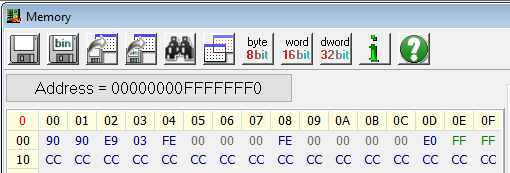
\includegraphics[scale=0.8]{Images/UEFI/ResetVector1}
	\end{center}
	\item First thing that BIOS does, is to get to Protected Mode.
	\begin{center}	
\begin{tikzpicture} [x=0.8cm,y=-0.8cm]
\tikzmath{
	\Gap = 0.2;
}
\draw (0,0) rectangle (3,1) node [pos=0.5] {Processor};
\draw (0,2) rectangle (3,10);
\draw (0 + \Gap,2 + \Gap) rectangle (3 - \Gap, 5.5) node [pos=0.5] {MCH};
\draw (0 + \Gap,6.5) rectangle (3 - \Gap, 10 - \Gap) node [pos=0.5] {Intel ICH9};
\draw (0,11) rectangle (3,12);
\draw (4,2) rectangle (15,4) node [pos=0.5] {System Memory};
\draw[fill=green!50] (13,2) rectangle (15,4) ;

\draw[fill=green!50] (4,8) rectangle (6,10) node [pos=0.5] {SPI Flash} ;

\foreach \x in {8.4, 8.8, 9.2, 9.6}
{
	\draw (6, \x-0.1) rectangle (6+\Gap, \x+0.1);
	\draw (4-\Gap, \x-0.1) rectangle (4, \x+0.1);
}

\draw[style = dashed] (6,8) -- (13,4);
\draw[style = dashed] (6,10) -- (15,4);
\draw[style = dashed] (15-\Gap, 2) -- (15-\Gap,4);

\draw[<->] (1.5, 1) -- (1.5,2+\Gap);
\draw[<->] (3 - \Gap,9) -- (4,9);
\draw[<->] (3 - \Gap,3) -- (4,3) node [above] {{\tiny Channel A}};
\draw[<->] (1.5, 10 - \Gap) -- (1.5,11) node [pos=0.5] {LPC I/F};
\draw[<->] (1, 5.5) -- (1,6.5) node [above left] {{\tiny DMI Interface}};
\draw[<->] (2, 5.5) -- (2,6.5) node [above right] {{\tiny Controller Link}};

\draw[->,color=red,line width =1pt] [out=0] (3,0.5) to [in=90] (15-\Gap,2) node[above right]{0xFFFFFFF0};
\node [below] at (4,4) {0x00000000};
\node [below right] at (15,4) {0xFFFFFFFF};
\end{tikzpicture}
\end{center}
\end{itemize}

\end{note}
\section{System Management Mode}
\begin{note}[General notes]:
\begin{itemize}
	\item SMM is a special execution mode of IA-32 architecture that was introduced with i386, chapter 34 of \href{http://www.intel.com/content/www/us/en/processors/architectures-software-developer-manuals.html}{Intel 64 and IA-32 Architectures Software Developer’s Manual}
	\item Some time ago SMM was used by BIOS developers mostly for power management and legacy devices emulation, for example, PS/2 support (port 60h/64h) for USB keyboard and mouse. Nowadays it's also widely used for firmware and platform security purposes.
	\item SMM executable code and data lives inside SMRAM and when SMRAM is locked — it can't be accessed by code of operating system or user mode software. System firmware (legacy BIOS or UEFI) copies SMM code into SMRAM and locks it during platform initialization.
	\item Processor is switching to SMM only trough System Management Interrupt (SMI), it saving current execution context into SMRAM and start executing SMI handler that can exit from SMM and resume execution from saved context using RSM instruction.
	\item System Management Interrupt has the highest priority and can’t be masked. Most important facts about SMI handler execution environment:
	\begin{enumerate}
		\item Similar to 16-bit real address mode with paging disabled.
		\item CS segment base is SMRAM base, EIP is 8000h.
		\item Segment limits are set to 4 GBytes, you can switch to protected mode or long mode to access all of the physical memory.
		\item All I/O ports are available.
		\item SMM code can read or modify saved execution context.
		\item SMM code can set it’s own IDT and use software interrupts.
	\end{enumerate}
	\item There’s a several ways to generate SMI:
	\begin{enumerate}
		\item Ring 0 code can trigger software SMI at any time by writing some byte value to APMC I/O port B2h.
		\item Internal chipset registers (\verb|SMI_EN|, \verb|GEN_PMCON_1| and others) that accessible via PCI config space allows to enable or disable different kind of hardware SMI sources.
		\item You can route hardware interrupts into SMM by reconfiguring of advanced programmable interrupt controller (APIC) that integrated into CPU.
		\item I/O instruction restart CPU feature (chapter 34.12 of IA-32 Architectures Software Developer’s Manual) allows to generate SMI on any I/O port access by \verb|IN| or \verb|OUT| processor instruction.
	\end{enumerate}
	\item SMRAM can be located in Compatible Memory Segment (CSEG), High Memory Segment (HSEG) or Top of Memory Segment (TSEG) system memory regions.
\end{itemize}
\end{note}